\subsection{The complex}
\label{sec:complex}

\todo{write something about topology}

% \begin{defin}
%   \(K\) is called a \emph{cube complex}, if it is a \(M_0\)-polyhedral complex, where every cell \(C\) is given by a unit cube of arbitrary dimension.
% \end{defin}

% From now on, if not otherwise specified, all cells \(C\) will be taken to be cubes.

% \begin{lemma}
%   \label{lemma:cube-dist}
%   Let \(x \leq C\) a cell and \(\dim C > 0\). Then
%   \begin{align*}
%     d(x, C - \st(x)) =
%     \begin{cases}
%       1 & \text{if } \dim \supp(x) = 0\\
%       d(x, \partial \supp(x)) & \text{else}
%     \end{cases}
%                          .
%   \end{align*}
% \end{lemma}

% \begin{proof}
%   If \(l = 0\) then \(x\) is a vertex of \(C^k\) and any other vertex (which exist, as \(k > 0\)) has distance at least \(1\) and is by definition not contained in the star of \(x\). Hence, \(d(x, C^k - \st(x)) \leq 1\).
  
%   After a rotation of the cube, we may assume that \(x\) is the origin and hence any face \(F\) of \(C^k\), not containing \(x\) must have at least one \(\delta_i = 1\). Let \(n_F\) denote the sum of all \(\delta_i\) defining \(F\). Then for all \(y \in F\), we have
%   \begin{align*}
%     d(x,y) = |y| \geq n_F \geq 1
%   \end{align*}
%   if \(x\) is not contained in \(F\). \(C^k - \st(x)\) is compact, therefore there there exists a \(y \in C^k - \st(x)\), such that
%   \begin{align*}
%     d(x, C^k - \st(x)) = d(x, y) 
%   \end{align*}
%   holds. Furthermore, there must exist a face \(F\) containing \(y\) in its interior. By definition of \(y\), \(F\) cannot contain \(x\). Together with the above argument we yield \(d(x, C^k - \st(x)) \geq 1\), which proves the first assertion.

%   Now, let \(l\) be different from \(0\). After a rotation, we can identify \(F\) with \(C^l\). \(\partial C^l \subset C^k - \st(x)\) holds and thus we have
%   \begin{align}
%     \label{eq:dist-border}
%     d(p, C^k - \st(x) \leq d(x, \partial C^k) < 1 .
%   \end{align}
%   As above, we find a \(y \in C^k - \st(x)\), realizing the distance. \(y\) lies in the interior of some face \(G\) and, by definition, \(G\) does not have \(C^l\) as a face. First, let us assume that \(G \cup \partial C^l \neq \varnothing\). In that case there is a unique projection \(\hat y \in G \cup \partial C^l\) of \(y\) and an element \(y_\perp\) orthogonal to \(C^l\), such that \(y = \hat y + y_\perp\). Then we have
%   \begin{align*}
%     d^2(x, y) = |x - \hat y|^2 + |y_\perp|^2 \leq d(x, \hat y).
%   \end{align*}
%   Hence \(y_\perp = 0\), which leads to \(y = \hat y \in \partial C^l\). If \(G \cup \partial C^l = \varnothing\), then at least one of the components \(l+1, \dots, k\) have to be fixed to \(1\), leading to \(d(x, C^k - \st(x)) = d(x,y) \geq 1\), which is a contradiction to Equation~\ref{eq:dist-border}, which proves the other inequality.
% \end{proof}

% \begin{lemma}
%   If \(K\) is a cube complex, then \(\epsilon(x) > 0\) (c.\,f.~\eqref{eq:epsilon}) for arbitrary \(x \in K\).
% \end{lemma}

% \begin{proof}
%   By definition of a cube complex, for any point \(x\) and two preimages \(x_i \in C_{\lambda_i}\), we have an isometry \(h \colon \supp(x_1) \to \supp(x_2)\). Hence, for any \(F_i \leq C_{\lambda_i}\), we have that \(d(x_1, F_1 \setminus \st(x_1)) = d(x_2, F_2 \setminus \st(x_2))\) by Lemma~\ref{lemma:cube-dist}. This shows that \(d(x, C \setminus \st(x))\) can be computed in any preimage of the cell \(C\) and furthermore, that the value is independent of \(C\). Hence, \(\epsilon(x) > 0 \).
% \end{proof}

In the following is a short list of deeper results about cube complexes, which we will need in the following, but which we will not be able to prove. The interested reader may find the results in~\cite[Appendices A, B]{MR3029427}. For the finite dimensional case we refer to~\cite[Sec. I.7, II.5]{MR1744486}.

\begin{thm}[{\cite[I.7.10]{MR1744486}}]
  If \(X\) is a cube complex, then \(d\) is a metric.
\end{thm}

% \begin{proof}
%   The symmetry in triangle enequality follow directly from the definition. It remains to prove that \(d(x,y) = 0\) implies \(x = y\). In order to do that, we claim that if \(d(x,y) < \epsilon(x)\), then there exists a cube \(C \subset K\), such that \(x, y \in C\) with preimages \(\bar x, \bar y \in C_\lambda\) such that \(d(x,y) = d_{C_\lambda}(\bar x,\bar y)\). The claim then follows directly. However, we will not show this claim directly but further reduce the assertion. We consider \(m\)-strings \(s \coloneqq (x_0, \dots, x_m) \in K^{m+1}\), with the property that each sucessive pair of points \(x_{i-1}, x_i\) are contained in a common cube \(C_i\). With this we define the length of a string as \(l(s) = \sum_{i=1}^n d_{C_i}(x_{i-1}, x_i)\), where \(d_{C_i}\) is the metric on \(C_i\) induced by any of its preimages under the natural projection.

%   These \(m\)-strings are in \(1:1\)-correspondence with piecwiese geodesic segments in \(K\) and thus we can use the two notions interchangeable. We will prove the claim: If \(l(s) < \epsilon(x_0)\), then there exists a cube \(C \subset K\) with \(x_0, x_m \in C\) and such that \(d_C(x_0, x_m) \leq l(s)\). We proceed by induction. For \(m=1\) the claim is true by definition. Assume that the claim is true for some \(m \in \N\) and let \(s = (x_0, \dots, x_{m+1})\) be an \((m+1)\)-string and \(s'\) the \(m\)-string consisting of the first \(m+1\) entries. By definition there exists a cube \(C\) such that \(x_m, x_{m+1} \in C\). Furthermore, \(d(x_0, x_m) \leq l(s') \leq l(s) < \epsilon(x_0)\). Hence, \(x_m \in \st(x_0)\). So there exists a second cube \(\tilde C\) that contains \(x_m\) in its interior. Also \(\tilde C \cap C\) is not empty and hence also a cube. Since \(x_m\) is in the interior of \(\tilde C\) we have \(\tilde C \subset C\) and hence \(x_0 \in C\). We have
%   \begin{align*}
%     d_C(x_0, x_{m+1}) \leq d_C(x_0, x_m) + d_C(x_m x_{m+1}) \stackrel{\ast}{\leq} l(s') + d_C(x_m + x_{m+1}) = l(s),
%   \end{align*}
%   which is what we wanted to show. For the inequality \(\ast\), we use the induction hypothesis together with the observation that if the inequality is true for any cube containing \(x_0\) and \(x_m\), then it is true for all cubes containing both points.

%   So we see that for all pairs \(x,y \in K\) with \(d(x,y) < \epsilon(x)\), we find a cube \(C\) containing both and \(d_C(x,y) \leq d(x,y)\). However, by construction of \(d\) this already implies equality. For \(d_C\) we already know that it is a metric on its cube. So \(d(x,y) = 0\) implies \(x = y\).
% \end{proof}


\begin{thm}[{\cite[Thm A.6]{MR3029427}}, {\cite[Thm I.7.50]{MR1744486}}]
  A cube complex is complete if and only if every chain of ascending cubes is finite.
\end{thm}


\begin{defin}[Flag complex]
  A \emph{flag complex} \(K\) is a simplicial complex, such that each complete subgraph of its 1-skeleton of \(n\) vertices, spans a \(n-1\) simplex in \(K\).
\end{defin}

\begin{thm}[Gromov's link condition, {\cite[Thm B.8]{MR3029427}}, {\cite[Thm II.5.20]{MR1744486}}]
  \label{thm:link}
  A cube complex \(K\) is \emph{non-positively curved} if and only if \(\lk(v,K)\) of each vertex \(v \in K\) is a flag complex.

  A cube complex \(K\) is \emph{CAT(0)} if and only if \(\lk(v,K)\) of each vertex \(v \in K\) is a flag complex and \(K\) is simply connected.
\end{thm}

\begin{bsp}
  \todo{add examples}
  \begin{itemize}
  \item trees
  \item graphs (NPC)
  \item tori
  \item surfaces
  \item products of \(X \times Y\) of cube complexes \(X,Y\)
  \end{itemize}

  % Torus
  \begin{tikzpicture}
    [vertex/.style={circle,fill=black, minimum size=1mm, inner sep=0pt}]
    \draw [>-   ] (-2, 2) -- (-1, 2) (-1, 2) -- ( 0, 2);
    \draw [>-   ] (-2,-2) -- (-1,-2) (-1,-2) -- ( 0,-2);
    \draw [>>-  ] ( 0, 2) -- ( 1, 2) ( 1, 2) -- ( 2, 2);
    \draw [>>-  ] ( 0,-2) -- ( 1,-2) ( 1,-2) -- ( 2,-2);
    \draw [>={Stealth},>- ] ( 2,-2) -- ( 2,-1) ( 2,-1) -- ( 2, 0);
    \draw [>={Stealth},>- ] (-2,-2) -- (-2,-1) (-2,-1) -- (-2, 0);
    \draw [>={Stealth},>>-] ( 2, 0) -- ( 2, 1) ( 2, 1) -- ( 2, 2);
    \draw [>={Stealth},>>-] (-2, 0) -- (-2, 1) (-2, 1) -- (-2, 2);
    \draw [dashed] ( 0, 2) -- ( 0,-2);
    \draw [dashed] ( 2, 0) -- (-2, 0);
    \node at ( 0, 0) [vertex,draw,label= 45:\(x\)] {};
    \node at ( 2, 0) [vertex,draw,label=135:\(z_1\)] {};
    \node at (-2, 0) [vertex,draw,label= 45:\(z_1\)] {};
    \node at ( 0, 2) [vertex,draw,label=315:\(z_2\)] {};
    \node at ( 0,-2) [vertex,draw,label= 45:\(z_2\)] {};
    \node at ( 2, 2) [vertex,draw,label=225:\(y\)] {};
    \node at (-2,-2) [vertex,draw,label= 45:\(y\)] {};
    \node at (-2, 2) [vertex,draw,label=315:\(y\)] {};
    \node at ( 2,-2) [vertex,draw,label=135:\(y\)] {};
  \end{tikzpicture}
  % \hfill{}
  \hspace{2cm}
  % link of torus
  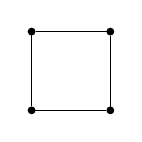
\begin{tikzpicture}
    [
    vertex/.style={
      circle,
      fill=black,
      minimum size=1mm,
      inner sep=0pt
    }
    ]
    \node at (0,0) [vertex] {}
    edge (0,1)
    node at (0,1) [vertex] {}
    edge (1,1)
    node at (1,1) [vertex]{}
    edge (1,0)
    node at (1,0) [vertex]{}
    edge (0,0);
  \end{tikzpicture}
  % Genus 2
  \begin{tikzpicture}
    [
    vertex/.style={
      circle,
      fill=black,
      minimum size=1mm,
      inner sep=0pt
    },
    ->-/.style={
      decoration={
        markings,
        mark=at position 0.4 with {\arrow{#1}}
      },
      postaction={decorate}
    }
    ]
    \node (1) at ( 2, 0) [vertex, label=0:\(y\)] {};
    \node (2) at ( 1.41, 1.41) [vertex, label=45:\(y\)] {}
    edge [bend right, ->-=>] (1);
    \node (3) at ( 0, 2) [vertex, label=90:\(y\)] {}
    edge [bend right, ->-=>>] (2);
    \node (4) at (-1.41, 1.41) [vertex, label=135:\(y\)] {}
    edge [bend right, ->-=<] (3);
    \node (5) at (-2, 0) [vertex, label=180:\(y\)] {}
    edge [bend right, ->-=<<] (4);
    \node (6) at (-1.41,-1.41) [vertex, label=225:\(y\)] {}
    edge [bend right, ->-={Stealth}] (5);
    \node (7) at ( 0,-2) [vertex, label=270:\(y\)] {}
    edge [bend right, >=Stealth, ->-={>>}] (6);
    \node (8) at ( 1.41,-1.41) [vertex, label=135:\(y
    \)] {}
    edge [bend right, >=Stealth, ->-={<}] (7)
    edge [bend left,>=Stealth, ->-={>>} ] (1);
    \node at (22.5:1.6) [vertex, label=22.5:\(z_1\)] {}
    edge [dashed] (202.5:1.6)
    node at (202.5:1.6) [vertex, label=202.5:\(w_1\)] {};
    \node at (67.5:1.6) [vertex, label=67.5:\(z_2\)] {}
    edge [dashed] (247.5:1.6)
    node at (247.5:1.6) [vertex, label=247.5:\(w_2\)] {};
    \node at (112.5:1.6) [vertex, label=112.5:\(z_1\)] {}
    edge [dashed] (292.5:1.6)
    node at (292.5:1.6) [vertex, label=292.5:\(w_1\)] {};
    \node at (157.5:1.6) [vertex, label=157.5:\(z_2\)] {}
    edge [dashed] (337.5:1.6)
    node at (337.5:1.6) [vertex, label=337.5:\(w_2\)] {};
    \node at ( 0, 0) [vertex,label=45:\(x\)] {};
  \end{tikzpicture}
  % link of genus 2
  \begin{tikzpicture}
    [
    vertex/.style={
      circle,
      fill=black,
      minimum size=1mm,
      inner sep=0pt
    }]
    \node at (0,0) [vertex] {}
    edge (1,0)
    node at (1,0) [vertex] {}
    edge (1,1)
    node at (1,1) [vertex] {}
    edge (1,2)
    node at (1,2) [vertex] {}
    edge (1,3)
    node at (1,3) [vertex] {}
    edge (0,3)
    node at (0,3) [vertex] {}
    edge (0,2)
    node at (0,2) [vertex] {}
    edge (0,1)
    node at (0,1) [vertex] {}
    edge (0,0);
    \node at (2,0) [vertex] {}
    edge (3,0)
    node at (3,0) [vertex] {}
    edge (3,1)
    node at (3,1) [vertex] {}
    edge (2,1)
    node at (2,1) [vertex] {}
    edge (2,0);
  \end{tikzpicture}
  % Sphere
  \begin{tikzpicture}
    [
    vertex/.style={
      circle,
      fill=black,
      minimum size=1mm,
      inner sep=0pt
    },
    ->-/.style={
      decoration={
        markings,
        mark=at position 0.5 with {\arrow{#1}}
      },
      postaction={decorate}
    }
    ]
    \node ( 1) at ( 0, 0) [vertex] {};
    \node ( 2) at ( 0, 1) [vertex] {};
    \node ( 3) at ( 1, 0) [vertex] {};
    \node ( 4) at ( 1, 1) [vertex] {};
    \node ( 5) at ( 0, 2) [vertex] {};
    \node ( 6) at ( 1, 2) [vertex] {};
    \node ( 7) at ( 0, 3) [vertex] {};
    \node ( 8) at ( 1, 3) [vertex] {};
    \node ( 9) at (-1, 1) [vertex] {};
    \node (10) at (-1, 2) [vertex] {};
    \node (11) at ( 2, 1) [vertex] {};
    \node (12) at ( 2, 2) [vertex] {};
    \node (13) at ( 3, 1) [vertex] {};
    \node (14) at ( 3, 2) [vertex] {};
    \draw[->-=>] (0,0) -- (1,0);
    \draw[->-=>>] (1,0) -- (1,1);
    \draw[->-=<<] (1,1) -- (2,1);
    \draw[->-=<] (2,1) -- (3,1);
    \draw[>={Stealth}, ->-=>] (3,1) -- (3,2);
    \draw[>={Stealth}, ->-=>>] (3,2) -- (2,2);
    \draw[>={triangle 45}, ->-=>] (2,2) -- (1,2);
    \draw[>={triangle 45}, ->-=<] (1,2) -- (1,3);
    \draw[>={Stealth}, ->-=<<] (1,3) -- (0,3);
    \draw[>={triangle 45}, ->-=>>] (0,3) -- (0,2);
    \draw[>={triangle 45}, ->-=<<] (0,2) -- (-1,2);
    \draw[>={Stealth}, ->-=<] (-1,2)-- (-1,1);
    \draw[>={open triangle 45}, ->-=>] (-1,1) -- (0,1);
    \draw[>={open triangle 45}, ->-=<] (0,1) -- (0,0);
    \draw (0,1) -- (1,1) -- (1,2) -- (0,2) -- (0,1);
    \draw (2,2) -- (2,1);
  \end{tikzpicture}
  % link of sphere
  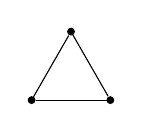
\begin{tikzpicture}
    [
    vertex/.style={
      circle,
      fill=black,
      minimum size=1mm,
      inner sep=0pt
    }]
    \node at (0,0) [vertex] {}
    edge (1,0)
    node at (1,0) [vertex] {}
    edge (0.5, 0.87)
    node at (0.5, 0.87) [vertex] {}
    edge (0,0);
  \end{tikzpicture}
\end{bsp}

\begin{defin}[Morphisms of cube complexes]
  \label{def:morphism-ccc}
  Let \(X,Y\) be cube complexes. \(f\colon X \to Y\) is called a \emph{morphism of cube complexes} or a \emph{combinatorial map}, if
  \begin{enumerate}
  \item each vertex \(v \in X^{(0)}\) is mapped to a vertex \(f(v) \in Y^{(0)}\),
  \item each cube \(C \subset X\) is mapped to a cube \(f(C) \subset Y\) and
  \item the induced map given by
    \[
      f_{\lambda, \omega}\colon C_\lambda \xrightarrow{p_{X,\lambda}} C \xrightarrow{f} f(C) \xrightarrow{p^{-1}_{Y,\omega}} C_\omega
    \]
    can be represented as \(f_{\lambda,\omega}(x) = \sum_{i=1}^n a_i f(v_i)\), where \(v_1, \dots, v_n\) are the vertices of \(C_\lambda\) and \(x = \sum_{i=1}^n a_i v_i\) is an arbitrary element of \(C_\lambda\) in its convex representation.
  \end{enumerate}
  \(\Aut(X)\) will denote the automorphism group of a cube complex \(X\).
\end{defin}

\begin{rem}
  The above definition of a combinatorial map is completely analogous to the one of a simplicial map (confere for example~\cite{Singer}).
\end{rem}

\begin{lemma}
  After possibly rotating \(C_\lambda \subset \R^n\) and \(C_\omega \subset \R^m\) \(f_{\lambda, \omega}\) is induced by the restriction of the natural projection from \(\R^n\) to \(\R^m\). In particular we have \(n \geq m\).
\end{lemma}

\begin{cor}
  \(f_C\colon C \to Y\) is distance non-increasing for each cube \(C \subset X\).
\end{cor}

\begin{prop}
  Let \(f\colon X \to Y\) be a combinatorial map. Then \(f\) is distance non-increasing, i.\,e.\ \(d_Y(f(x), f(y)) \leq d_X(x,y)\) for all \(x,y \in X\). In particular a combinatorial isomorphism is an isometry.
\end{prop}

\begin{proof}
  By the combinatorial structure of \(f\) each piecewise linear path \(c\) in \(X\) is mapped to a piecewise linear path in \(Y\). For each \(x,y \in X\) we denote by \(\operatorname{PL}(x,y)\) the piecewise linear paths joining \(x\) to \(y\). Furthermore, each segment of \(c\) lying in a cube is shortened by the previous corollary. Hence, \(l(f \circ c) \leq l(c)\) and thus
  \begin{align*}
    d_X(x,y)
    & = \inf\left\{l(c) \relmid c \in \operatorname{PL}(x,y)\right\}\\
    & \geq \inf\left\{l(f \circ c) \relmid c \in \operatorname{PL}(x,y)\right\}\\
    & \geq \inf\left\{l(c) \relmid c \in \operatorname{PL}(f(x), f(y))\right\}\\
    & = d_Y(x,y),
  \end{align*}
  which is the desired result.
\end{proof}

\begin{lemma}
  Let \(f\colon X \to Y\) be a combinatorial map and a local homeomorphism between cube complexes. Then \(f|_C\colon C \to f(C)\) is an isometry for every cube \(C \subset X\) and \(f\) is a local isometry.
\end{lemma}

\begin{proof}
  For the first assertion consider \(x \in \mathring{C}\) and a open neighborhood \(U\) of \(x\) such that \(f|_U\) is a homeomorphism. Let \(v_1, \dots, v_n \in C\) be the vertices of \(C\). Then, using these coordinates, we can write \(x = \sum_i a_i v_i\) with \(a_i\) coefficients of the convex combination and \(f\) takes the form
  \[
    f(x) = \sum_i a_i f(v_i).
  \]
  Assume that \(f(v_1), \dots, f(v_n)\) are not pairwise different. That means without loss of generality we have \(f(v_1) = f(v_2)\). Let \(\epsilon > 0\) and define
  \[
    y \coloneqq \sum_i b_i v_i \quad \text{with } b_i = \begin{cases}a_1 + \epsilon & i = 1\\a_2 - \epsilon & i = 2\\ a_i & \text{else}\end{cases}.
  \]
  Since \(U\) is open and \(x \in \mathring{C}\), we can choose \(\epsilon\) small enough such that \(y \in U \cap C\), but by construction we have \(f(y) = f(x)\), which is a contradiction to the fact that \(f|_U\) is homeomorphism. Hence the \(f(v_i)\) need to be pairwise differnt, but this is already sufficient to show that \(f|_C\) is an isometry.

  For the second claim consider \(z \in X\). Then there exists an \(\epsilon(z)\) such that each \(y \in in B(z, \epsilon(z))\) and \(z\) lie in a common cube (c.\,f.~\cite[I.7.8-9]{MR1744486}) and by \textcite[I.7.33]{MR1744486} we have that it is always positve. Let \(0 < \epsilon \leq \epsilon(z)\), such that \(f\) is a homeomorphism \(B \coloneqq B(z, \epsilon)\). Set \(\tilde B \coloneqq f(B)\) and let \(\tilde x, \tilde y \in \tilde B \cap \tilde C\), where \(\tilde C\) is some cube in \(Y\). Then we find unique preimages \(x\) and \(y\) in \(B\).
  Assume there is no common cube containing both \(x\) and \(y\).
  Let us consider the case that \(\tilde x \in \supp(\tilde y) \subset \tilde C\) and consider \(C = \supp(y)\) and \(C' = \supp(x)\). Then \(f|_C\colon C \xrightarrow{\sim} \supp(\tilde y)\). Hence, there exists \(x' \in C\), such that \(f(x') = \tilde x\). Furthermore, \(x\) and \(y\) lie both in \(B\) yielding that \(z \in C \cap C'\). We consider the two straight line segments \(c\) and \(c'\) connecting \(x\) and \(x'\) to \(z\) respectively. Since \(f\) is combinatorial \(f \circ c\) and \(f \circ c'\) are also straight line segments in a common cube. Both segments have identical endpoints and therefore must coincide. However, except for the endpoint \(z\) the segments \(c\) and \(c'\) need to be disjoint as they lie in the interior of \(C\) and \(C'\) respectively. Additionally at some point they will enter \(B\). However, this leads to a contradiction regarding the injectivity of \(f\) on \(B\).

  The case where \(y \in \supp(x)\) can be handeld analogously. So lastly, consider the case where neither \(y\) lies in \(\supp(x)\) nor \(x\) lies in \(\supp(y)\). Without loss of generality replace \(\tilde C\) by the smallest cube containing both \(\tilde x\) and \(\tilde y\) (and hence both their supports). Assume there is no cube \(C\) in \(X\) containing \(\supp(y)\) which is mapped to \(\tilde C\). Then \(f\) cannot be a local homeomorphism, because its image can never be open. Hence, the \(C\) must exist and thus also a \(x' \in C\) with \(f(x') = \tilde x\). Choosing \(C' = \supp(x)\), the same reasoning as in the first case can be applied which again leads to a contradiction.

  All in all it was established that if \(\tilde x, \tilde y \in \tilde B \cap \tilde C\) then there exists a cube \(C \subset X\) such that the preimages \(x, y\) both lie in it. However, this already shows that any piecewise linear path in \(\tilde B\) is mapped to a piecewise linear path in \(B\) by \(f^{-1}\).

  As a last step, choose \(\epsilon(\tilde z) > \delta > 0\), \(\tilde W \coloneqq B(\tilde z, \delta) \subset B\) and \(W \coloneqq f^{-1}(\tilde W) \subset B\). Then \(\tilde W\) is convex\todo{cite source}\ and for any two points \(\tilde x, \tilde y \in \tilde W\) we find a geodesic \(c\) joining the two in \(\tilde W\). By the previous assertion \(f^{-1} \circ c\) is also a piecewise linear path, which has also the same length as \(f\) is an isometry on cubes. Thus we have
  \begin{align*}
    d_Y(f(x), f(y))
    & = d_Y(\tilde x, \tilde y)\\
    & = l(c)\\
    & = l(f^{-1} \circ c)\\
    & \geq d_X(x,y).
  \end{align*}
  Since we already established that \(f\) is distance non-increasing, this shows that \(f\) is an isometry on \(W\).
\end{proof}

\begin{prop}
  \label{prop:covering}
  Let \(p \colon \tilde X \to X\) be a covering map between topological spaces and let \(\tilde X\) be connected. If \(X\) is a cube complex, then \(\tilde X\) can be given a cube complex structure, such that \(p\) becomes a combinatorial map. In particular, with this structure on \(\tilde X\), \(p\) becomes a local isometry.
\end{prop}

\begin{proof}
  Consider the embeddings \(p_\lambda\colon C_\lambda \to X\), \(v_\lambda \coloneqq p_\lambda(0)\) and \(F_\lambda \coloneqq p^{-1}(\{v_\lambda\})\). Then for each \(f \in F_\lambda\) we yield a unique lift \(p_{\lambda, f}\colon C_\lambda \to \tilde X\).
  Doing this for each \(\lambda\) we construct a map
  \[
    \pi \colon \bigcup_{\lambda \in \Lambda} \bigcup_{f \in F_{\lambda}} C_\lambda \times {\lambda, f} \to \tilde X.
  \]
  This \(\pi\) is surjective and open. Additionally, all the lifted maps \(p_{\lambda, f}\) are injective. So as a last step to show that this \(\pi\) defines a cube complex structure on \(\tilde X\) one needs to see that the gluing is realized by isometries. So take \(x \in C_\lambda\) and \(y \in C_{\lambda'}\) such that \(p_{\lambda,f}(x) = p_{\lambda', f'}(y)\). This also implies that \(p_\lambda(x) = p_{\lambda'}(y)\). Since \(X\) is a cube complex we find an isometry \(\phi\colon \supp(x) \to \supp(y)\) such that \(p_{\lambda'} \circ \phi  = p_\lambda\). Consider
  \[
    A \coloneqq \{z \in \supp(x) \mid (p_{\lambda', f'} \circ \phi)(z) = p_{\lambda, f}(z)\}.
  \]
  Then \(A \neq \varnothing\) as \(x\) lies in \(A\). Next consider a sequence \((z_n)_{n \in \N} \subset A\) with \(\lim_{n \to \infty} z_n = z \in \supp(x)\). Then \(p_\lambda(z_n) = (p_{\lambda'} \circ \phi)(z_n)\) by construction and hence the same is true for \(z\) by continuity (in a metric space). However, then we find a open neighborhood \(U\) of \(p_{\lambda,f}(z)\) such that \(p|_U\) is a homeomorphism on its image and hence we have
  \begin{align*}
    p_{\lambda,f}(z)
    & = ((p|_U)^{-1} \circ p \circ p_{\lambda,f})(z)\\
    & = ((p|_U)^{-1} \circ p_\lambda)(z)\\
    & = ((p|_U)^{-1} \circ p_{\lambda'} \circ \phi)(z)\\
    & = ((p|_U)^{-1} \circ p \circ p_{\lambda',f'} \circ \phi)(z)\\
    & = (p_{\lambda', f'} )(z).
  \end{align*}
  This shows that \(A\) is closed. Lastly consider any \(z \in A\). Then there exists a neighborhood \(U\) of \(p_{\lambda, f}(z)\) such that \(p|_U\) is a homeomorphism on its image. Let \(w \in V \coloneqq p_{\lambda, f}^{-1}(U)\). Then
  \begin{align*}
    p_{\lambda,f}(w)
    & = ((p|_U)^{-1} \circ p \circ p_{\lambda,f})(w)\\
    & = ((p|_U)^{-1} \circ p_\lambda)(w)\\
    & = ((p|_U)^{-1} \circ p_{\lambda'} \circ \phi)(w)\\
    & = ((p|_U)^{-1} \circ p \circ p_{\lambda', f'} \circ \phi)(w)\\
    & = (p_{\lambda', f'} \circ \phi)(w)
  \end{align*}
  and \(A\) is open. The space \(\supp(x)\) is connected so this implies \(A = \supp(x)\) and thus the gluing is indeed realized by isometries.

  With this \(\tilde X\) is a cube complex and by construction \(p\) is a combinatorial map. Together with the previous lemma this yields that \(p\) is a local isometry.
\end{proof}

\begin{cor}
  With the notation of the previos proposition, it holds that \(\dim X = \dim \tilde X\).
\end{cor}


\begin{defin}
  A cube complex \(X\) is called \emph{locally finite} if every \(x \in X\) is contained in only finitely many cubes. It is called \emph{locally compact} if for every \(x \in X\) there exists a compact neighborhood \(K \subset X\). It is called \emph{locally countable} if every \(x \in X\) is contained in at most countably many cubes.
\end{defin}

\begin{prop}[{\cite[Prop.~14]{Rolli2012}}]
  Let \(X\) be a cube complex. Then the following are equivalent:
  \begin{enumerate}
  \item \(X\) is locally finite,
  \item Each bounded subset of \(X\) meets only finitely many cubes,
  \item \(X\) is proper (i.\,e.\ closed balls are compact) and
  \item \(X\) is locally compact.
  \end{enumerate}
\end{prop}

\begin{lemma}
  \label{lem:lf-countable}
  If \(X\) is a locally countable CAT(0) cube complex. Let \(V(X)\) be its vertex set considered with the edge metric \(d\). Then for every \(x_0 \in V(X)\) and \(n \in \N_0\)the sets \(X_n \coloneqq \{x \in V(X) \mid d(x_0, x) = n\}\) are countable.
\end{lemma}

\begin{proof}
  We fix \(x_0 \in V(X)\) and proceed by induction. \(X_0 = \{x_0\}\) since \(d\) is a metric. Now, assume \(X_n\) to be countable and let for each \(x \in V(X)\) be \(N(x)\) the set of its neighboring vertices (i.\,e.\ all vertices connected by an edge to \(x\) or equivalently all vertices with distance 1 from \(x\)). Because of the local countability \(N(x)\) is countable. Thus
  \[
    X_{n+1} \subset \bigcup_{x \in X_n} N(x)
  \]
  is a countable set.
\end{proof}

\begin{bsp}
  \todo{examples for visual boundary}
\end{bsp}

\begin{rem}
  From now on we will assume that all our complexes are connected, locally countable and finite-dimensional.\todo{Add remark that non-elementarity implies unboundedness}
\end{rem}

%%% Local Variables:
%%% mode: latex
%%% TeX-master: "../Master"
%%% End:
